\section{Balanceo de cargas}
Esta sección creo que merecía estar en la parte final del complemento ya que es una mirada hacia un futuro. Por lo que después de él no hay nada.
\\La escalabilidad de las aplicaciones web ha conseguido mucha representatividad en los últimos tiempos. Podemos ver sitios web gigantescos y acceder a ellos desde todas las partes del mundo.
\\Tenemos ejemplos como Google, Amazon, Facebook. Empresas que sus sitios webs lo son todo y que sin ellos no hubieran cogido la relevancia que han tenido durante todo este tiempo.
\\La escalabilidad la considero un concepto de relevancia debido a que los sistemas tienden a crecer y a ampliarse, siendo optimistas claros. No sabemos si en cuarenta años los docentes y estudiantes se habrán quintuplicado en el Departamento de Informática y en sintonía el uso de la aplicación.
\\Si todo este argumento no convence creo que es mejor recurrir al viejo y clásico: ``Mejor prevenir que curar''.

\subsection{Docker Swarm}
Docker Swarm es una funcionalidad que nos brinda Docker que nos permite gestionar los recursos de nuestros contenedores agrupándolos en un cluster.
\\Esta característica nos ayuda a poder distribuir la carga de trabajo de una aplicación en la red de forma rápida y ahorrando tiempo y recursos de nuestros contenedores. Toda esta gestión se realizaría de forma centralizada.
\\La arquitectura de Swarm es maestro-esclavo. Es decir, cada clúster está formado al menos por un nodo maestro y tantos nodos esclavos como queramos. Mientras que el maestro se encarga de gestionar el clúster y delegar tareas el esclavo se encarga de ejecutar las unidades de trabajo. Como ejemplo pongamos la COVID-19.
\\La COVID supuso un aumento de las infraestucturas red en tiempo récord. Tanto supuso este incremento del uso de internet que había varios momentos al día que este dejaba de funcionar durante un tiempo.
\\Ahora pasemos el ejemplo de infraestucturas red de una página web como la del Aula Virtual de la Universidad de Almería. Esta página implementó un servicio externo para poder realizar videoconferencias que utilizaban bastantes universidades españolas.
\\En un principio todo iba perfecto, ya que se preparó el sistema para una carga grande pero entonces llegó la época de exámenes y la historia se cuenta sola.
\\Una herramienta magnífica que nos ayuda a soportar cargas altas o simplemente distribuir recursos para que unas máquinas no se vean sobrecargadas es Docker Swarm.

\subsection{¿Cómo podemos implementar Docker Swarm?}
Primero de todo necesitamos poder crear otra máquina virtual en nuestra cuenta de Google Cloud. La primera máquina la ubicamos en Estados Unidos pero esta vez la ubicaremos en Finlandia. La configuración la podremos ver en la figura \ref{fig:creando-segunda-maquina}.
\begin{figure}
    \centering
    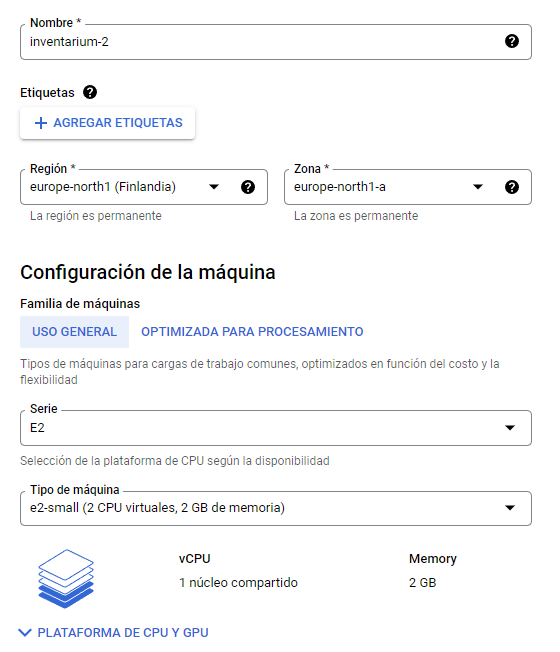
\includegraphics[scale=0.6, keepaspectratio]{imagenes/complemento/docker-swarm/creating_second_virtual_machine.png}
    \caption{Creando segunda máquina virtual}\label{fig:creando-segunda-maquina}
\end{figure}
\\Las dos máquinas virtuales que tendríamos en nuestro entorno Cloud serían las que podemos ver en la figura \ref{fig:entorno-maquinas-cloud}.
\begin{figure}
    \centering
    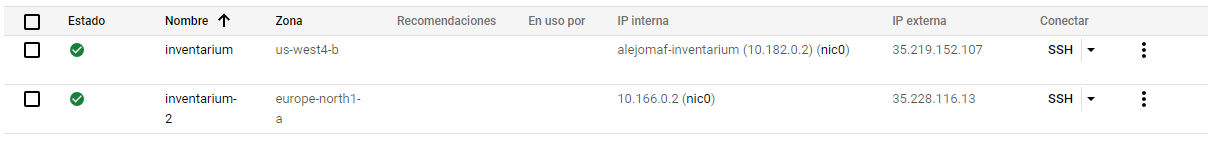
\includegraphics[scale=0.45, keepaspectratio]{imagenes/complemento/docker-swarm/virtual_machines_on_google_cloud.png}
    \caption{Entorno de máquinas en Google Cloud}\label{fig:entorno-maquinas-cloud}
\end{figure}
\\Procederemos a configurar y a instalarle Docker.
\\Cuando ya lo tengamos instalado iremos a nuestra máquina principal que queremos que actúe como líder, ejecutaremos el siguiente comando que vemos en la figura \ref{fig:docker-swarm-init}.
\begin{verbatim}
    sudo docker swarm init
\end{verbatim}
\begin{figure}
    \centering
    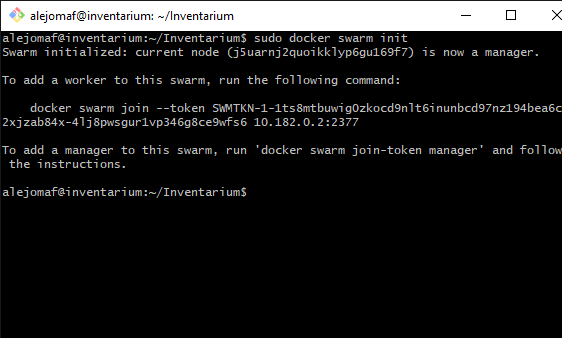
\includegraphics[scale=0.5, keepaspectratio]{imagenes/complemento/docker-swarm/docker-swarm-init.png}
    \caption{Inicializando el entorno de docker swarm}\label{fig:docker-swarm-init}
\end{figure}
Esto nos generará un token para poder añadir un nodo a nuestro clúster de contenedores. Para poder ingresar a él escribiremos el comando que nos indica Docker tal como se muestra en la figura \ref{fig:docker-compose-join}.
\begin{figure}
    \centering
    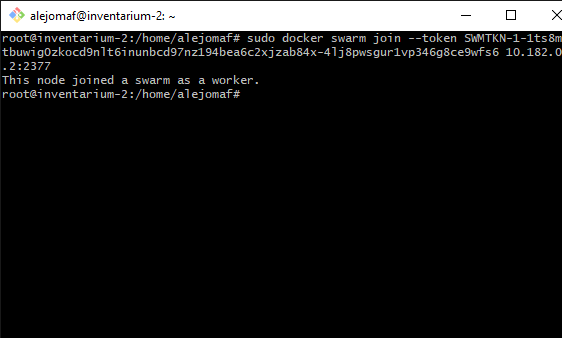
\includegraphics[scale=0.5, keepaspectratio]{imagenes/complemento/docker-swarm/docker-compose-join.png}
    \caption{Añadiendo nodo esclavo a nuestro entorno}\label{fig:docker-compose-join}
\end{figure}
Con esto ya tendríamos nuestro swarm creado. Podemos añadir tantas máquinas como queramos a ella.

\subsection{¿Cómo desplegar nuestro entorno en Docker Swarm?}
Para poder realizar el despliegue ejecutaremos el siguiente comando dentro de nuestro nodo maestro. Para ello necesitaremos disponer del \textit{docker-compose.yml} que hemos generado en el proyecto. Desde el directorio de la aplicación donde se encuentra ubicado el fichero ejecutamos:
\begin{verbatim}
    sudo docker stack deploy --compose-file docker-compose.yml inventarium
\end{verbatim}
Inventarium es el nombre que tendrá nuestro deploy y del que luego haremos referencia. Podemos ver el proceso de creación en la figura \ref{fig:docker-stack-deploy}.
\begin{figure}
    \centering
    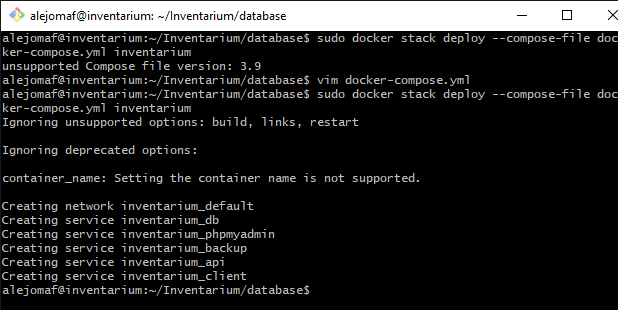
\includegraphics[scale=0.5, keepaspectratio]{imagenes/complemento/docker-swarm/docker-stack-deploy.png}
    \caption{Deploy de nuestro entorno Docker en el clúster}\label{fig:docker-stack-deploy}
\end{figure}
A partir de este punto surgió una problemática y es que al analizar las máquinas que estaban ejecutándose dentro de nuestro swarm observé que había una que no llegaba a crearse.
\\Esta máquina era la de nuestro servidor personalizado con Node. El contenedor con el cual tuvimos que realizar una configuración personalizada con un Dockerfile para que su configuración fuera correcta.
\\Lo que ocurría era que su máquina al no estar publicada en DockerHub esta no se podía descargar desde ningún lado de nuestro nodo esclavo por lo que teníamos que publicar nuestra imagen.
\\Primero de todo tenemos que iniciar sesión en Docker con:
\begin{verbatim}
    sudo docker login
\end{verbatim}
Luego construiremos nuestra imagen con el Dockerfile, para poder publicarla en DockerHub el nombre de la imagen tiene que seguir la estructura \textit{nombre\_usuario/nombre\_imagen:version} ejecutando el siguiente comando en la terminal:
\begin{verbatim}
    sudo docker build -t alejomaf/inventarium_api:1.0 .
\end{verbatim}
Al generar nuestra imagen lo que nos quedaría es subirla a DockerHub y eso lo conseguimos ejecutando:
\begin{verbatim}
    sudo docker push alejomaf/inventarium_api:1.0
\end{verbatim}
Volveremos a ejecutar nuestro deploy y obtendremos el maravilloso resultado de la figura \ref{fig:docker-swarm-final}.
\begin{figure}
    \centering
    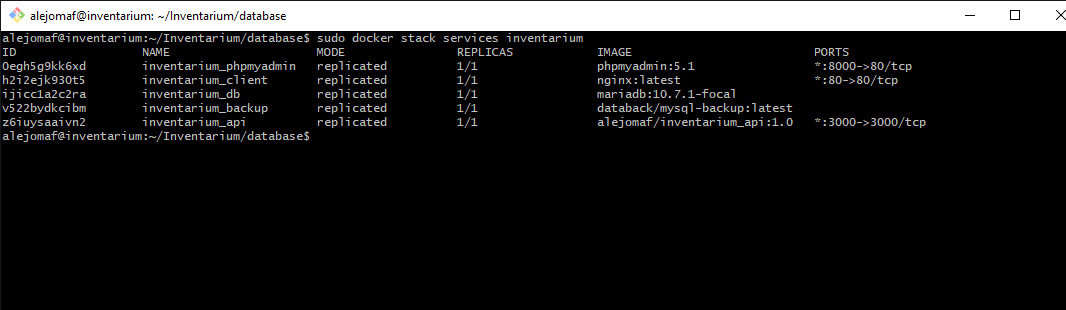
\includegraphics[scale=0.4, keepaspectratio]{imagenes/complemento/docker-swarm/docker-FINAL.png}
    \caption{Visualización de los servicios corriendo en Docker Swarm}\label{fig:docker-swarm-final}
\end{figure}

